\chapter{ Truy xuất nguồn gốc thực phẩm dựa trên công nghệ Blockchain}
\section{Đặt vấn đề}

Như đã trình bày ở chương \ref{Chapter2}, ta cần tìm ra một mô hình có thể đảm bảo 
tính toàn vẹn và đáng tin cậy cao, khó bị tấn công từ bên ngoài, và giúp 
cải thiện tính minh bạch và đáng tin cậy trong quá trình sản xuất và vận 
chuyển sản phẩm.  

Bài toán truy xuất nguồn gốc thực phẩm là một trong những ứng dụng tiềm năng của công nghệ 
blockchain. Bằng cách sử dụng blockchain, thông tin về nguồn gốc, vận chuyển và lưu trữ 
của các sản phẩm thực phẩm có thể được lưu trữ và truy xuất một cách an toàn và minh bạch.
\subsection{Ưu điểm mô hình truy xuất nguồn gốc thực phẩm dựa trên blockchain}
 
\begin{itemize}
    \item \textbf{Minh bạch:} Các thông tin về nguồn gốc, vận chuyển và lưu trữ của các sản phẩm 
    thực phẩm được lưu trữ và truy xuất một cách an toàn và minh bạch.
    \item \textbf{An toàn:} Các thông tin về nguồn gốc, vận chuyển và lưu trữ của các sản phẩm 
    thực phẩm được lưu trữ và truy xuất một cách an toàn và minh bạch.
    \item \textbf{Đáng tin cậy:} Các thông tin về nguồn gốc, vận chuyển và lưu trữ của các sản phẩm 
    thực phẩm được lưu trữ và truy xuất một cách an toàn và minh bạch.
\end{itemize}

\subsection{Cách tiếp cận và giải pháp}

Sử dụng nền tảng Hyperledger Fabric để xây dựng một mạng lưới blockchain phù hợp với 
mục đích truy xuất nguồn gốc thực phẩm.

\section{Mô hình hệ thống}
\subsection{Các thành phần tham gia}

Cốt lõi của hệ thống được thực hiện dưới dạng chaincode. Chaincode cung cấp các thao tác cho phép người dùng hệ thống thêm và sửa đổi 
thông tin trong blockchain một cách an toàn và có thể theo dõi được. Người sử dụng hệ thống
là các thành viên chuỗi cung ứng và các bộ phận quản lý. Các thực thể tham gia 
vào hoạt động của hệ thống là các tổ chức người dùng, trong đó mỗi người dùng được xác định 
bằng một chứng chỉ do cơ quan chứng nhận liên kết với tổ chức được xác định rõ ràng mới có thể 
tham gia vào các hoạt động của hệ thống. Trong Hyperledger Fabric, tập hợp các tổ chức tham 
gia vào các hoạt động blockchain được xác định trước. Hyperledger Fabric cho phép thêm một tổ 
chức mới hoặc xóa một tổ chức hiện có trong thời gian chạy bằng cách chuyển một loạt các 
giao dịch sang blockchain phải được đa số các tổ chức tham gia chấp thuận.

Với hệ thống truy xuất nguồn gốc thực phẩm, thành viên bao gồm: 
\begin{itemize}
    \item[-] Nhà cung cấp giống vật tư: Dữ liệu truy tìm bao gồm thông tin về nguyên liệu 
    thực phẩm nông nghiệp (ví dụ: hạt giống, thuốc trừ sâu và phân bón), giao dịch với người nông dân v.v.
    \item[-] Nông dân: Dữ liệu truy tìm bao gồm thông tin về các trang trại, quá trình canh tác,
    điều kiện thời tiết, giao dịch với các nhà sản xuất, ...
    \item[-] Nhà sản xuất: Dữ liệu truy tìm bao gồm thông tin về các nhà máy, quá trình sản xuất,
    giao dịch với nông dân và nhà phân phối,...
    \item[-] Công ty vận chuyển: Dữ liệu truy tìm bao gồm chi tiết vận chuyển, điều kiện lưu trữ, giao
    dịch với nông dân, nhà phân phối hay nhà sản xuất,...
    \item[-] Nhà phân phối: Dữ liệu truy tìm bao gồm thông tin về các cửa hàng, quá trình phân phối,
    ngày nhập hàng, hạn sử dụng, các giao dịch với nhà sản xuất,...
\end{itemize}

Tuỳ vào từng sản phẩm cụ thể, mô hình có thể thêm hoặc bớt các thành viên tham gia. 
\subsection{Phân tích và thiết kế hệ thống}
\subsubsection{Domain Model}

\begin{figure}[h]
    \centering
    \includegraphics[width=0.7\textwidth]{images/domain_model.png}
    \caption{Domain Model của Business Logic \cite{app}} 
\end{figure}

Các tổ chức muốn tham gia vào chuỗi cung ứng sẽ đăng ký tham gia. Để được xác nhận, 
tổ chức sẽ kí hợp đồng thông minh thể hiện qua chaincode. Nếu thoả mãn hợp đồng, 
tổ chức sẽ được thêm vào và có một mã định danh ID. Chaincode thể hiện các điều khoản
và các cam kết cần thực hiện. 

Một loại sản phẩm muốn thêm vào blockchain sẽ được đăng ký thông qua một hợp đồng 
thông minh. Nó thoả mãn các yêu cầu thì sẽ được thêm vào blockchain. Việc kiểm tra 
yêu cầu này được thực hiện một cách tự động thông qua các hàm của chaincode. Sản phẩm có một 
số thuộc tính như ID, type, state,...
Một sản phẩm có thể được cấu tạo từ nhiều nguyên liệu, vật tư,... Những nguyên liệu ấy
có thể đã được tồn tại trong mạng blockchain. Nếu tồn tại trong mạng blockchain, ta sẽ thêm 
thuộc tính params để thể hiện mối quan hệ. Nếu không thì ta sẽ yêu cầu giao dịch
để ghi thông tin về sản phẩm. 

Việc xây dựng Domain Model như này giúp việc quản lý nguồn gốc cũng như xác thực nguồn gốc 
dễ dàng hơn, như quản lý được sản phẩm được sản xuất từlô nông sản nào, cũng từ đó truy xuất được nguồn gốc giống của sản phẩm nôngsản.
\subsubsection{Chaincode (Hợp đồng thông minh)}
Chaincode nó được sử dụng để xác định các đầu vào và đầu ra của các giao dịch trên blockchain. Chaincode là một chương trình được 
viết bằng một trong các ngôn ngữ lập trình.

Một số hàm tiêu biểu của chaincode trong hệ thống truy xuất nguồn gốc thực phẩm.

\begin{itemize}
    \begin{figure}[h]
        \centering
        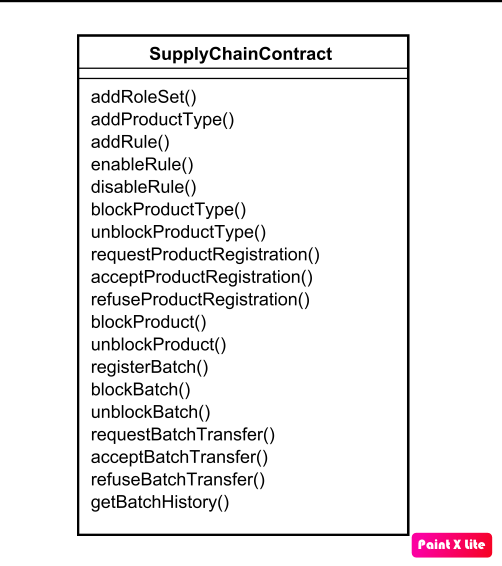
\includegraphics[width=0.4\textwidth]{images/Smart_Contract.png}
        \caption{Chaincode \cite{app}}
    \end{figure}
    \item \textbf{addRoleSet():} Thêm một thành viên mới vào hệ thống. Thành viên này có thể là một tổ chức hoặc cá nhân.
    \item \textbf{addProductType():} Thêm một loại sản phẩm mới vào hệ thống. Loại sản phẩm này có thể là sản phẩm chính hoặc sản phẩm phụ.
    \item \textbf{addRule():} Thêm một quy tắc mới vào hệ thống. Quy tắc này có thể là quy tắc chính hoặc quy tắc phụ.
    \item \textbf{enableRule () và disableRule ():} Cho phép bật và tắt rule qua ruleId.
    \item \textbf{blockProductType() và unblockProductType():} cho phép chặn và mở chặn một loại sản phẩm.
    \item \textbf{requestProductRegistration():} yêu cầu đăng ký một sản phẩm mới.
    \item \textbf{acceptProductRegistration() và refuseProductRegistration():} cho phép chất nhận hoặc từ chối đăng ký sản phẩm.
    \item \textbf{blockProduct() và unblockProduct():} cho phép chặn và mở chặn một sản phẩm.
    \item \textbf{registerBatxh():} cho phép một tổ chức đăng ký một lô sản phẩm liên kết với sản phẩm nào đó.
    \item \textbf{blockBatch() và unblockBatch():} cho phép chặn và mở chặn một lô sản phẩm.
    \item \textbf{requestBatchTransfer():} cho phép một tổ chức yêu cầu chuyển một lô sản phẩm từ một tổ chức khác.
    \item \textbf{acceptBatchTransfer() và refuseBatchTransfer():} cho phép chấp nhận hoặc từ chối chuyển lô sản phẩm.
    \item \textbf{getBatchHistory():} cho phép lấy lịch sử của một lô sản phẩm.
\end{itemize}
\subsubsection{Tạo mạng}
\subsection{Các bước thực hiện}
Các bước thực hiện cơ bản của hệ thống truy xuất nguồn gốc thực phẩm như sau:
\begin{itemize}
    \item[-] \textbf{Bước 1:} Các tổ chức đăng ký thành viên vào hệ thống.
        \item[-] \textbf{1.1:} Các tổ chức tạo nút thành viên. 
        \item[-] \textbf{1.2:} Các nút thành viên tham gia vào kênh.
        \item[-] \textbf{1.3:} Tổ chức tạo admin là nút khách trong hệ thống, và yêu cầu
        tham gia vào kênh. Peer node xác thực thông tin của client và cấp quyền.
    \item[-] \textbf{Bước 2:} Các tổ chức đăng ký các loại sản phẩm của riêng mình bằng cách 
    gửi yêu cầu giao dịch. Các bước thực hiện được trình bày ở \ref{subsec:luonggiaodich} của chương \ref{chap:hyper}.
    \item[-] \textbf{Bước 3:} Các tổ chức lần lượt thêm các thông tin, các thông tin sẽ được
    lưu trữ trong các khối nối tiếp nhau và sắp xếp theo thời gian. Các nút thành viên sẽ lưu 
    trữ chuỗi khối này ở sổ cái.
    \item[-] \textbf{Bước 4:} Khách hàng đăng nhập vào ứng dụng và nhập mã để yêu cầu truy xuất
    thông tin sản phẩm. Nếu sản phẩm chỉ thuộc 1 kênh, không có nguyên liệu thuộc kênh
    khác thì sẽ trả về thông tin sản phẩm. Ngược lại thì sẽ truy xuất thông tin nguyên liệu
    của sản phẩm đó và trả về tất cả thông tin sản phẩm.
\end{itemize}


\section{Công nghệ sử dụng}
- Docker

- Golang

- Hyperledger Fabric

\section{Thực nghiệm}

\section{Kết luận và hướng phát triển}